\documentclass[runningheads]{llncs}
\usepackage[T1]{fontenc}
\usepackage[utf8]{inputenc}
\usepackage{graphicx}
\usepackage{booktabs}
\usepackage{amsmath,amssymb}
\usepackage{tikz}
\usetikzlibrary{positioning,arrows.meta}
\usepackage{microtype}
\usepackage[hidelinks]{hyperref}
\renewcommand\UrlFont{\color{black}\rmfamily}
\def\UrlBreaks{\do\/\do\.\do\-\do\@}
\Urlmuskip=0mu plus 2mu\relax

\newcommand{\F}{macro-$F_1$}

\begin{document}

\title{Interpretable Stylometric Features with Automatic Difficulty Routing for Sentence-Level Author Switch Detection}
\titlerunning{Interpretable Author Switch Detection}

\author{Tshephang Phuti-A-Nkutu Matlala\orcidID{0009-0002-0058-6016}}
\authorrunning{T. P. Matlala}
\institute{University of Johannesburg, South Africa\\
\email{223004635@student.uj.ac.za}}

\maketitle

\begin{abstract}
Author switch detection asks, for every pair of adjacent sentences in a document, whether the author changed. The strongest current systems are fine-tuned transformers, which are accurate but hard to explain. We study how far an interpretable alternative goes. Each sentence is described by 63 named stylometric features and three hashed profiles (characters, parts of speech, function words), and each pair of sentences by z-scored differences and distances between profiles. A decision tree, a logistic regression and a small neural network classify the pair. Because the three difficulty levels of the benchmark have very different base rates of change, a detector recognises the level of a document and selects its decision threshold. Trained on all 2.44 million training pairs and evaluated on a held-out half of the labelled validation split of the PAN 2026 multi-author data, the three classifiers reach an overall macro-$F_1$ of 0.710--0.712 with one threshold (0.462 for always predicting `no change') and 0.719--0.729 with level-specific thresholds. The detector names the right level for 88.8\,\% of documents, and an ablation of 52 neural-network runs shows highly redundant feature groups. The scores lie well below those of transformer systems and are not official test-set results; the contribution is a reproducible, readable baseline with its limits stated.

\keywords{Author switch detection \and Style change detection \and Stylometry \and Interpretable machine learning \and Multi-author writing style analysis}
\end{abstract}

%% ---------------------------------------------------------------------------------------------------------------
\section{Introduction}

A text written by several people changes voice where one writer takes over from another. The Multi-Author Writing Style Analysis (MAWSA) task at PAN has moved from asking whether a document has one author or several, to locating changes between paragraphs, and now to the finest grain: given two adjacent sentences, decide whether the author changed~\cite{zangerle2020overview,bevendorff2021overview,zangerle2025overview,zangerle:2026}. In 2026 the documents are English fan fiction in three difficulty levels, and the official score is the macro-averaged $F_1$ over all pairs of a level~\cite{zangerle:2026,bevendorff:2026b}. The strongest systems fine-tune DeBERTa-family transformers and score near 1.0 on easy and about 0.77 on medium and hard documents~\cite{zangerle:2026}.

We did not try to beat them: we want a system whose every input is a named, countable property of the text, so that a reader can ask which property moved a decision, and we ask how much signal is left without a pre-trained language model.

Transparent features matter in practice. In an academic-integrity or forensic case, a flag that two passages differ in authorship is only useful if someone can say \emph{why}, and a score from a language model rarely allows that. Interpretable systems are also cheap: ours trains and runs on CPU. What is missing is evidence of how much accuracy this transparency costs at sentence level, and of where it fails.

This paper provides that evidence, on the sentence-level benchmark of the PAN 2026 shared task. We ask three questions. \textbf{RQ1:} how far do interpretable features and small models go when trained on all the data? \textbf{RQ2:} the levels have base rates of about 30\,\%, 5\,\% and 21\,\% changes; does a level-aware threshold, chosen by an automatic difficulty detector, help? \textbf{RQ3:} which feature groups carry the signal, and which are redundant? Our contributions are a complete from-scratch pipeline trained and evaluated on the full data, a difficulty detector with a per-level threshold router, an ablation of feature groups and hyper-parameters, and a critique that separates what the evidence supports from what it does not. Section~\ref{sec:related} reviews related work, Section~\ref{sec:methods} describes the method, Section~\ref{sec:results} reports the results, and Section~\ref{sec:discussion} discusses their limits.

%% ---------------------------------------------------------------------------------------------------------------
\section{Literature Review}
\label{sec:related}

\paragraph{The task.} The unit of prediction in style change detection has shrunk over the years of the PAN shared tasks, from whole documents through the number of authors and the paragraph of a change~\cite{zangerle2020overview,bevendorff2021overview} to the sentence-level setting with difficulty levels of 2025 and 2026~\cite{zangerle2025overview,zangerle:2026}; the lab overview places it among the other PAN tasks~\cite{bevendorff:2026b}.

\paragraph{Classical stylometry.} Writers differ in habits they do not control. Mosteller and Wallace separated the disputed Federalist Papers by the rates of common function words~\cite{mosteller1964inference}, and Burrows' Delta compares texts through z-scored frequencies of frequent words~\cite{burrows2002delta}. Later work compares learners over such features for attribution~\cite{10.1093/llc/fqq001}. Readability formulas~\cite{flesch1948new,gunning1952technique,kincaid1975derivation} were designed for another purpose but are cheap, interpretable numbers. Sentence-level feature sets~\cite{oloo2022optimal} and $n$-gram markers for literary text~\cite{rios2022detection} have also been studied.

\paragraph{Feature-based and neural systems.} Singh et al.\ describe paragraphs by character and part-of-speech $n$-grams, function words and vocabulary richness, and classify the absolute difference of two descriptions with logistic regression~\cite{singh2021writing}; our pair representation follows this idea. Others cluster feature vectors~\cite{alshamasi2022ensemble}, keep punctuation and special characters that are usually removed~\cite{zamir2024stylometry}, or, in a cheap and explainable pipeline of gradient-boosted trees on frequency-based features, tackle a different PAN task, the detection of AI-generated text~\cite{ochab2025styloch}. Neural systems use a contrastive style embedding~\cite{Chen2023AWS}, a natural-language-inference view of style change between paragraphs~\cite{kucukkaya2023arc}, fine-tuned RoBERTa on sentence pairs~\cite{rohra2025sentence}, a sequential sentence-pair classifier~\cite{schmidt2025team} and graph convolutional networks~\cite{alsheddi2025team}.

\paragraph{Gap.} Neural systems answer \emph{whether} a change happened, rarely \emph{which property of the text} made them say so. Feature-based studies answer this, but mostly on paragraphs, with one threshold and few ablations. To our knowledge, an automatic estimate of document difficulty used to choose a threshold, and a systematic leave-one-group-out ablation of an interpretable feature set, have not been examined at sentence level. This paper studies both.

%% ---------------------------------------------------------------------------------------------------------------
\section{Methods and Implementation}
\label{sec:methods}

Figure~\ref{fig:pipeline} shows the pipeline. All code is written in Java without machine-learning libraries, with a command-line runner and a Spring Boot interface. Code, scripts and logs are to be made available at \url{https://github.com/mat-tp/Author-Switch-Detection}.

\begin{figure}[t]
\centering
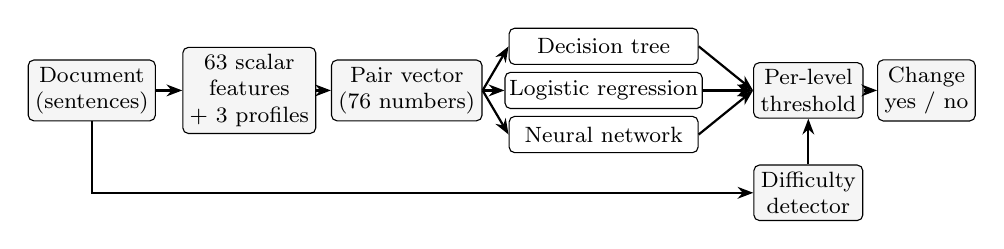
\begin{tikzpicture}[
  font=\footnotesize,
  box/.style={draw, rounded corners=2pt, align=center, minimum height=7mm, inner sep=2.5pt, fill=black!4},
  mod/.style={draw, rounded corners=2pt, align=center, minimum height=4.6mm, minimum width=24mm, inner sep=1.5pt, fill=white},
  arr/.style={-{Stealth[length=2mm]}, thick}]
  \node[box] (doc) at (0mm,0mm) {Document\\(sentences)};
  \node[box] (feat) at (20mm,0mm) {63 scalar\\features\\+ 3 profiles};
  \node[box] (pair) at (40mm,0mm) {Pair vector\\(76 numbers)};
  \node[mod] (m1) at (65mm,5.6mm) {Decision tree};
  \node[mod] (m2) at (65mm,0mm) {Logistic regression};
  \node[mod] (m3) at (65mm,-5.6mm) {Neural network};
  \node[box] (thr) at (91mm,0mm) {Per-level\\threshold};
  \node[box] (out) at (106mm,0mm) {Change\\yes / no};
  \node[box] (det) at (91mm,-13mm) {Difficulty\\detector};
  \draw[arr] (doc) -- (feat);
  \draw[arr] (feat) -- (pair);
  \foreach \m in {m1,m2,m3} {\draw[arr] (pair.east) -- (\m.west); \draw[arr] (\m.east) -- (thr.west);}
  \draw[arr] (thr) -- (out);
  \draw[arr] (doc.south) |- (det.west);
  \draw[arr] (det.north) -- (thr.south);
\end{tikzpicture}
\caption{The pipeline. Each pair classifier gives a score; the detector estimates the level of the document, and the threshold of that level turns the score into a decision.}
\label{fig:pipeline}
\end{figure}

\subsection{Data and Evaluation Protocol}

The MAWSA 2026 data~\cite{zangerle_2026_19068843,zangerle:2026} are English fan-fiction documents, 15\,000 per level, split 70/15/15 into training, validation and hidden test sets; each adjacent sentence pair has a binary label (1 = the author changes). All fitted parts (feature extractor with scaler and tables, models) see the \emph{training split only}: 31\,500 documents and 2\,439\,074 pairs, of which 347\,996 (14.27\,\%) are changes. The labelled validation split is cut \emph{by document} into two halves. The first (3\,375 documents) is used for every decision: early stopping, hyper-parameters and thresholds. The second, the \emph{held-out half} (3\,375 documents, 259\,653 pairs; change rates of 29.7\,\%, 4.5\,\% and 21.2\,\% on the easy, medium and hard levels), is used only for the reported scores. The score is the macro-$F_1$ of the classes `change' and `no change', as in the official metric, per level and over all pairs; thresholds maximise it on the first half. A system that never predicts a change scores 0.4128, 0.4886 and 0.4409 per level and 0.4622 overall (our reference line). \textbf{The held-out half is not the official hidden test set of the shared task; every number below comes from it and none is an official benchmark result.}

\subsection{Features and Their Motivation}

Features are grouped so that each group tests one idea, which the ablation needs. \emph{Length and word shape} (sentence length, word-length mean, spread and distribution): authors differ in how long their sentences and words are. \emph{Vocabulary} (type--token ratio, hapax share, Simpson's $D$, Yule's $K$, frequent-word share, TF-IDF, word rarity, an NRC emotion score~\cite{mohammad2013crowdsourcing}): how rich and unusual the wording is. \emph{Punctuation} (density, variety, the rate of twelve marks): largely unconscious, and fan-fiction writers differ strongly in dialogue marks, dashes and ellipses. \emph{Orthography and layout} (digits, capitals, ALL-CAPS, elongation, contractions, sentence start and end, spacing). \emph{Readability} (Flesch, Gunning Fog, Flesch--Kincaid), each compressing length and syllable counts into one number. \emph{Syntax} (shares of fifteen part-of-speech classes and their entropy, from a rule-based tagger written for this project): less tied to topic than vocabulary, which matters when topics are shared. Three \emph{profiles} complete the description, each a hashed bag of units~\cite{weinberger2009hashing}: character 3-grams (256 buckets), part-of-speech bigrams (128) and function words, the classical topic-independent marker~\cite{mosteller1964inference}. All 63 scalar features and all three profiles are used in every model.

\emph{Pair representation.} For two adjacent sentences, every scalar feature is z-scored with the training mean and standard deviation (as in Burrows' Delta~\cite{burrows2002delta}), clipped to $\pm 5$, and the absolute difference is taken. For each profile we add four distances between the two profile vectors: cosine, Jensen--Shannon~\cite{lin1991divergence}, total variation and Jaccard. One overall distance completes the vector: $63 + 3\times 4 + 1 = 76$ numbers.

\subsection{Classifiers and Their Settings}

The three pair classifiers span a range of readability and capacity; all weight the classes to offset the 14\,\% base rate. \textbf{Logistic regression} (10\,000 gradient steps, rate 0.6, no penalty) has one readable weight per column. The \textbf{decision tree}~\cite{breiman1984cart} (depth 5, at least 20 pairs to split, 5 per leaf) gives a rule path of at most five conditions. The \textbf{neural network} (76--128--64--32--16--8--1, Adam~\cite{kingma2015adam} rate 0.001, batch 64, dropout 0.2, L2 penalty 0.01, early stopping with patience 8; best epoch 16) is the only model that can use interactions between features. These settings are conventional defaults and were \emph{not} tuned; only thresholds and early stopping use the first validation half (Section~\ref{sec:ablation}: the L2 penalty matters, the architecture hardly).

\paragraph{An additional model.} As an exploratory extra, a small siamese network (32-dimensional embedding, triplet loss~\cite{schroff2015facenet}, window of one sentence) classifies a pair by the distance between embeddings. For cost reasons it was trained on a sample of 150\,000 sentences, about 6\,\% of the training documents, and it appears only in Table~\ref{tab:main}.

\subsection{Difficulty Detector and Threshold Router}

The base rates differ so much between levels that one threshold cannot suit all. The detector is a three-class softmax regression on 16 document-level numbers and their squares: topic similarity between sentences (cosine of content-word vectors), dispersion of the style features, and the logarithm of the number of sentences. It is trained, class-balanced, on the 31\,500 training documents. A \emph{router} applies the threshold tuned on the first validation half \emph{for the detected level}, and falls back to the pooled threshold if a file is missing. We compare four ways to choose the threshold: \emph{pooled} (one for all levels), \emph{true level} (an upper bound that needs the label), \emph{detected} (per document) and \emph{folder vote} (the level detected most often in a folder, applied to the whole folder, which suits an evaluation that delivers one level at a time).

%% ---------------------------------------------------------------------------------------------------------------
\section{Results and Analysis}
\label{sec:results}

All numbers are macro-$F_1$ on the held-out half, from one training run (one seed) per model.

\subsection{Main Results (RQ1)}

With one pooled threshold the three pair classifiers are nearly tied overall (Table~\ref{tab:main}: 0.7117 tree, 0.7098 logistic regression, 0.7113 neural network), 0.25 above the baseline; the additional retrieval model is lower overall (0.6619) but best on medium and hard documents. The gain is very unequal across levels. On easy documents the models are strong (0.91--0.92 pooled, 0.935--0.944 with the level's own threshold). On medium documents the three pair models are \emph{barely above the baseline} (0.501--0.508 against 0.489) at every setting. On hard documents the pooled threshold is also near the baseline (0.444--0.449 against 0.441); the real gain (0.538--0.553) appears only with the level's own threshold.

\begin{table}[t]
\caption{Macro-$F_1$ on the held-out half. Left: one threshold for all levels (pooled). Right: overall score for the other three ways to choose the threshold. Best per column in bold.}
\label{tab:main}
\centering
\setlength{\tabcolsep}{2.4pt}
\footnotesize
\begin{tabular}{lcccccccc}
\toprule
 & \multicolumn{4}{c}{pooled threshold} & \multicolumn{3}{c}{overall, other thresholds}\\
\cmidrule(lr){2-5}\cmidrule(lr){6-8}
Model & easy & med. & hard & all & detected & true level & folder vote\\
\midrule
Always `no change' & .4128 & .4886 & .4409 & .4622 & .4622 & .4622 & .4622\\
Decision tree & .9138 & .5011 & .4438 & \textbf{.7117} & .7073 & .7192 & .7192\\
Logistic regression & .9137 & .5075 & .4487 & .7098 & \textbf{.7187} & \textbf{.7285} & \textbf{.7285}\\
Neural network & \textbf{.9234} & .5052 & .4455 & .7113 & .7117 & .7221 & .7221\\
Retrieval (additional) & .8501 & \textbf{.5363} & \textbf{.4871} & .6619 & .7109 & .7216 & .7216\\
\bottomrule
\end{tabular}
\end{table}

\subsection{Does Knowing the Difficulty Help? (RQ2)}

Using the true level raises the overall score of every model (Table~\ref{tab:main}), from +0.008 for the tree to +0.019 for logistic regression. The gain sits in the hard level (tree: 0.4438 $\to$ 0.5530): the pooled threshold, tuned on all pairs, more than half of which are medium, is too strict for hard documents.

The detector is reliable but not perfect: its accuracy is 0.8877 on the held-out half (0.8821 on the first half, 0.8908 on a training sample, so it does not overfit). It recognises 883 of 1\,125 easy documents (202 are called hard), 1\,083 medium and 1\,030 hard (81 are called easy). Document by document, its choice beats the pooled threshold for logistic regression (+0.009), ties for the neural network (+0.0004) and is slightly worse for the tree ($-$0.004). The \emph{folder vote} named the right level for all three folders and so reproduces the true-level result exactly; it is the safer use of the detector when evaluation delivers one level at a time. One caution: the detector uses the number of sentences $n$, and the mean of $\ln(1+n)$ is 3.59, 4.80 and 3.78 for easy, medium and hard documents. Medium documents are longer, a property of how the dataset was built and not of the authors' style, so the detector may not transfer to differently built data.

\subsection{Which Features Matter? (RQ3)}
\label{sec:ablation}

We ran the neural network with each feature group removed in turn and alone, and swept its hyper-parameters. Only 52 of 120 planned runs finished in time: the complete feature-group study and these sweeps, but \emph{not} pipeline variants, other models or repeated seeds. With one seed, a difference below 0.01 is `within noise'. Table~\ref{tab:abl} shows the groups that carry signal.

\begin{table}[t]
\caption{Neural network, feature-group ablation on the held-out half. $\Delta$ = full model minus model without the group (positive: the group helps). `Alone' = the group by itself.}
\label{tab:abl}
\centering
\setlength{\tabcolsep}{3.5pt}
\footnotesize
\begin{tabular}{lrrrrrr}
\toprule
 & \multicolumn{2}{c}{without the group} & \multicolumn{4}{c}{group alone}\\
\cmidrule(lr){2-3}\cmidrule(lr){4-7}
Group & $\Delta$ all & $\Delta$ hard & all & easy & med. & hard\\
\midrule
All features & -- & -- & .7113 & .9435 & .5051 & .5439\\
Sentence length & +.0005 & +.0017 & .6566 & .8628 & .4966 & .4897\\
Flesch Reading Ease & +.0028 & $-$.0015 & .6844 & .8984 & .5002 & .4949\\
Gunning Fog & .0000 & $-$.0027 & .6731 & .8903 & .4968 & .4892\\
Flesch--Kincaid & $-$.0003 & $-$.0025 & .6752 & .9011 & .4961 & .4802\\
Per-mark punctuation & +.0001 & +.0273 & .5836 & .7221 & .5058 & .5281\\
POS shares & +.0018 & +.0041 & .5672 & .7061 & .5155 & .5385\\
\bottomrule
\end{tabular}
\end{table}

\emph{The groups are redundant.} Removing any one of the 18 groups moves the overall score by at most 0.003 (from $-$0.0016 to +0.0028), within noise.

\emph{Single groups are informative on easy documents and nearly empty on hard ones.} Sentence length alone gives 0.863 on easy documents and the readability indices 0.89--0.90 (baseline 0.413, full model 0.94). On hard documents the same groups reach 0.48--0.49, only a little above the 0.441 baseline and below the 0.5439 of the full model. The easy level can thus be solved largely with length-like measures, which fits its construction (changes that coincide with topic shifts); hard documents need several kinds of evidence together.

\emph{Punctuation matters on hard documents.} Removing the per-mark punctuation rates lowers the hard score by 0.027 (0.5439 to 0.5166), and removing punctuation density and variety by 0.008, although the overall score does not move. This fits the motivation of the group, but it rests on one seed. Ten groups (including both $n$-gram profiles and function words) give exactly the constant baseline alone; we believe this is a side effect of the L2 penalty of 0.01, which pushes weak features to zero (a penalty of 0.1 collapses the whole network to the constant prediction, 0.4622).

\emph{Hyper-parameters.} The L2 penalty is the only setting that matters. Chosen on the first half, the best penalty is 0 (validation 0.7379), giving 0.7294 on the held-out half (easy 0.9534, medium 0.5116, hard 0.5711), 0.018 above our default of 0.01 (0.7113). We report the default elsewhere because the other models were not re-run with the tuned value. Five hidden-layer layouts lie within 0.003 of each other, and dropout between 0 and 0.5 changes the overall score by less than 0.004.

%% ---------------------------------------------------------------------------------------------------------------
\section{Critique and Discussion}
\label{sec:discussion}

\paragraph{What the evidence supports.} With every training pair and every described feature, an interpretable pipeline reaches about 0.71 overall and 0.94 on easy documents, and a level-aware threshold lifts the overall score to 0.72--0.73, across four models and 259\,653 held-out pairs. Against the all-`no change' baseline the gain is clear on easy documents, clear on hard ones only once the threshold fits the level (0.54--0.57 against 0.441), and small on medium ones.

\paragraph{Distance to the state of the art.} The best systems of the 2026 shared task reach about 0.77 and 0.78 on medium and hard documents~\cite{zangerle:2026}; our 0.50--0.54 and 0.54--0.57 are far below, and the comparison is only indicative, since theirs come from the hidden test set. Medium is our weakest result: only 4.5\,\% of its pairs are changes, and a short sentence pair may hold too little evidence for any difference-based feature set; a neural model reading both sentences can use meaning and syntax together.

\paragraph{Is it interpretable?} The inputs are named, and the logistic regression and the tree can be read, but the pipeline does not yet explain a single prediction and we ran no user study. Because the groups are redundant, a weight or a split may be one of several equivalent choices; a faithful explanation would need, for example, permutation importance over groups. We claim a system that is \emph{transparent in its inputs}, not one that explains its decisions.

\paragraph{Threats to validity.} (1)~One seed: differences below 0.01 are ties. (2)~The ablation is partial (52 of 120 runs, neural network only), so redundancy may not hold for the other models. (3)~The held-out half comes from the validation split, not from the original PAN test data, and may be easier or harder. (4)~The POS features come from a rule-based tagger, so their weak showing may reflect tagger errors, not syntax. (5)~The detector partly uses document length. (6)~The default L2 penalty was not tuned.

%% ---------------------------------------------------------------------------------------------------------------
\section{Conclusion}

We asked how far an interpretable pipeline goes on sentence-level author switch detection. A pipeline of 63 named features and three profiles reaches an overall macro-$F_1$ of 0.71 on a held-out validation half and 0.94 on easy documents, but only about 0.50 on medium and 0.54--0.57 on hard documents, far from the transformer systems of the task. A difficulty detector that is right for 88.8\,\% of documents, used through a per-folder vote, recovers the gain of knowing the level (up to 0.7285 overall); this gave more than any change of classifier or architecture. The ablation shows redundant feature groups, a role for punctuation on hard documents and a large effect of an untuned L2 penalty.

The models were tested only on a held-out part of the labelled validation dataset. They should be tested on the original PAN at CLEF dataset, and the final reports are to be run through TIRA. Further work will finish the ablation for all models with several seeds, tune the L2 penalty, replace the rule-based tagger and add an explanation for each prediction.

\bibliographystyle{splncs04}
\bibliography{references}

\end{document}
